\section{Background}
Our work is related to the merging of ANN technology with more efficient Answer Set Programming languges. In this section we will provide a brief background on both subjects, motivating our work on C-MCPN.

\subsection{Artificial Neural Networks (ANNs)}
\textbf{Note:} \emph{As far as I can tell we are basically missing this section in the other paper(?), which we will need. In the other paper, section 2.3, there are a lot of citations and descriptions around the general subject, but nothing like ``here is the definition of an ANN as an example.''}

\subsubsection{Efficiency and Environmental Immpacts}

The introduction of big data (in particular by scraping the broader Internet) changed the landscape for AI, allowing statistical models to flex their strength, in particular because these models require massive amounts of data for  training purposes \parencite{Helm2020,Bhuyan2024}. This incredible need for information highlights an important drawback in the form of \emph{data efficiency} \parencite{Cropper2020}. This notable lack of efficiency translates to a significant need in terms of resources.

As an example, let us consider a the cost to train a single model, ChatGPT-3. According to DeVries \textbf{(et al.? I can't find the bib right now.)}, the training of GPT-3 required around 1.3 million kWh \emph{just} to be trained \parencite{DeVries2023}. With some quick, back-of-the-envelope calculations, we can put this into perspective. Consider that the average American household uses approximately 10,791 kWh per year \textbf{is the source EIA2025?}. Dividing these out we find that the model's energy use was proportional to:

\[1{,}300{,}000~\text{kWh} \times \frac{1~\text{household}}{10{,}791~\text{kWh/year}} \approx 120.5~\text{households}.\]

Similarly, we could produce a rough, \emph{lower bound} of how much water was likely used for training. A termoelectric power station can use approximately 43.8 L/kWh of water \parencite{Gordon2024}. That would put the \emph{indirect} water costs of training GPT-3 at approximately 56,940,000 L, approximated by:
\[1{,}300{,}000~\text{kWh} \times 43.8~\frac{\text{L}}{\text{kWh}} = 56{,}940{,}000~\text{L}\]%}

Given that an adult male averages approximately 4L of fresh water, that number represents sufficient water to sustain a lower bound of approximately 39,000 adults for a year \textbf{Citations needed: 4L., possible arithmetic needed to spell out 39K}. To put this number into perspective, this would likely be sufficient to provide fresh water to approximately the city of Brighton, CO, for a year.

Note that this figure includes {only} the indirect costs to generate the electricity--massive cooling costs for data center equipment would likely add significantly to our calculation. While these calculations are remarkably overly-simplified, we hope that it puts into perspective how the technology is already unsustainable. This highlights the dire need for more efficient AI and ML technologies \parencite{DeVries2023}. The discovery of models that are sufficiently sustainable to curb this resource use is an open problem.

We believe that one path towards a solution is to combine different AI methodologies, in particular those technologies that are known for higher efficiency. One possible candidate would be the use of satisfiability solvers, in particular modern Answer Set Programming languages, to accelerate the learning and inference processes.

\subsection{Answer Set Programming (ASP)}
Answer Set Programming serves as an amalgamation of Prolog-style (i.e., quantified logic) with powerful advances in satisfiability (SAT) solvers that occurred throught the 1990s and into the 2000s, expanding significantly in terms of the model sizes they are capable of processing and computational efficiency. In this section we will discuss the basic syntax and semantics of the ASP language, Clingo, which serves as a technological foundation of C-MPCN. \textbf{cite a relevant paper}.

\subsubsection{Syntax and Semantics}
The atomic units in an ASP dialect such as Clingo are \emph{literals}, which describe ideas and \emph{facts} that serve as statements that are held to be true. The basic syntax is the application of a \emph{property} to a literal, {\tt property(atom)}. E.g.,
\begin{verbatim}
red(apple).
\end{verbatim}
is a complete statement (and program), attributing a property of {red} to an idea named {\tt apple}. Such statements are \emph{purely declarative}, providing a \emph{description} of the problem (vs. specific processor instructions). I.e., we describe \emph{what} needs solving vs. \emph{how} to solve the problem in traditional imperative/algorithmic contexts.

Further knowledge is\emph{inferred} using aggregate statements known as \emph{rules}, taking the form: {\tt consequent :- antecedent}. This mirrors an \emph{implication} from formal logic, as the {\tt :-} symbol is read equivalently to $\leftarrow$. In such a statement the consequent \emph{must} be true whenever the antecedent is true. E.g., consider the statement:

\begin{verbatim}
  eat(Fruit) :- red(Fruit), ripe(Fruit).
\end{verbatim}

This describes a preference over what fruit will be eaten. I.e., ``If a fruit is red and ripe, then we eat the fruit.''

In this case rather than the literal {\tt apple}, we use a \emph{variable} to allow for inference. I.e., The {\tt Fruit} can be \emph{any} contextually-relevant literal in the program, so long as it possesses the required properties. Note that this functions differently from its analogous notion in imperative language--rather than a pattern to be matched variables typically serve as typed memory locations that are manipulated by the program.

%% \subsubsection{An Illustrative Example: 3-Colorability}
%% As an illustrative example regarding how to model problems in Clingo, we will use the graph 3-Colorability problem, as it is presented in \emph{ASP$\forall$: Answer Set Programming "Algorithms"} \textbf{Guerin et al., 2026--need cite}. The problem is in NP-Complete, meaning that while it is deceptively easy to state it is is computationally expensive to solve. A simplified statement of the problems is ``Given a graph, G, assign one of 3 colors to the vertices of G such that no two adjacent vertices share a color.''

%% E.g., Consider the following graph and solution:

%% \begin{figure}
%%   \begin{minipage}[t]{.49\linewidth}
%%     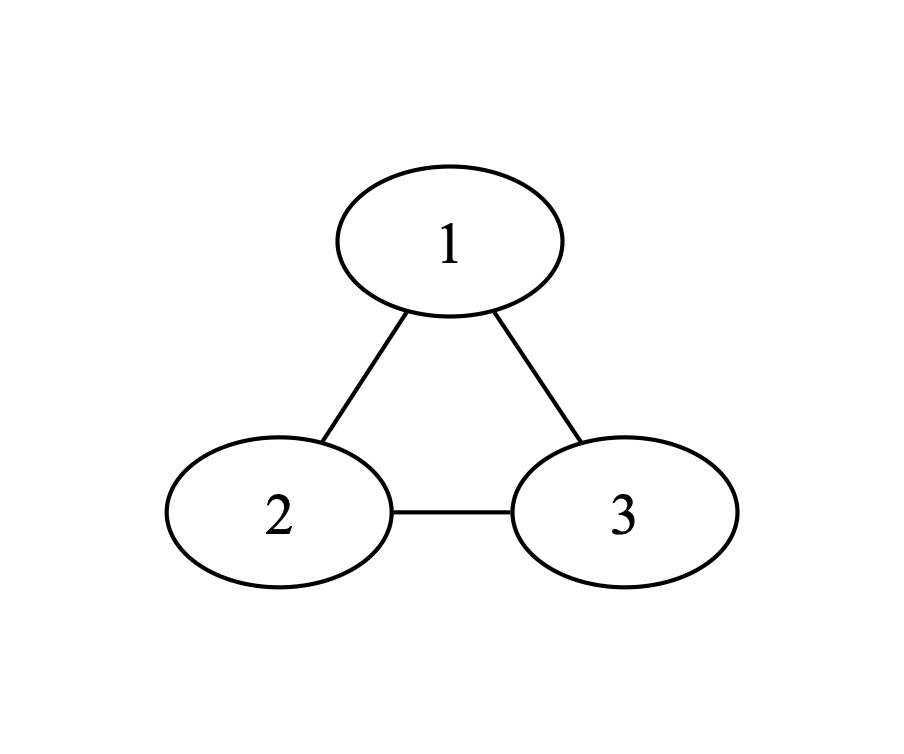
\includegraphics[scale=.15]{tex_files/sections/figures/graph}
%%   \end{minipage}
%%   \begin{minipage}[t]{.49\linewidth}
%%     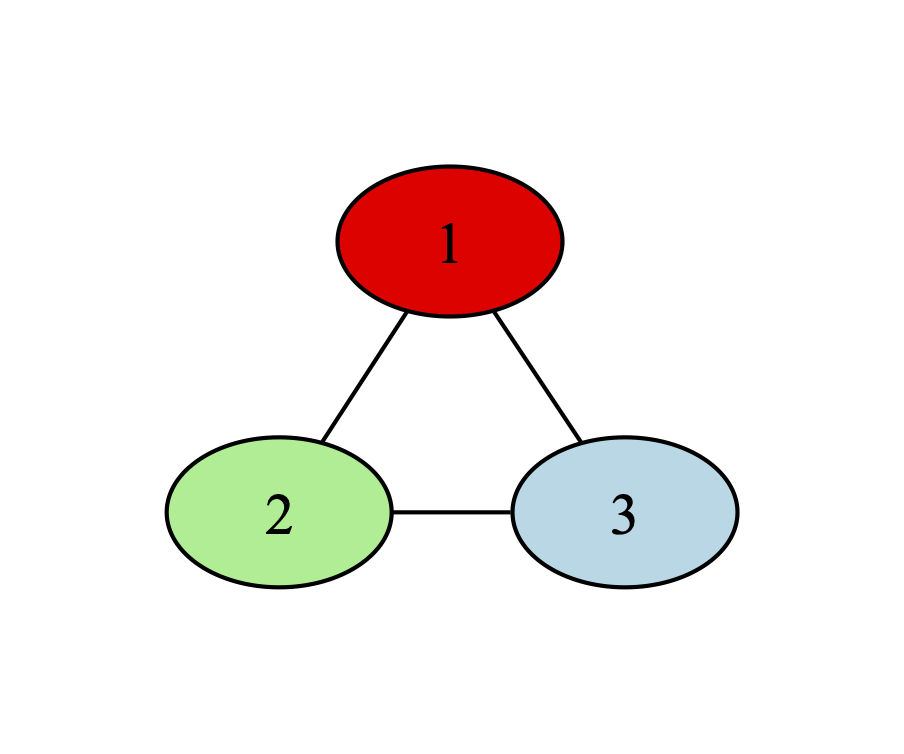
\includegraphics[scale=.15]{tex_files/sections/figures/graph_colored}
%%   \end{minipage}
%%   \caption{An Example Graph Coloring}\label{graph_color}
%% \end{figure}

%% While the example and coloring are rather trivial, we can see that under the provided assignment no two colors are connected by an edge.

%% In Clingo we specify the \emph{reasoning} behind the problem, and not the \emph{steps} required to find a solution (that is the work of the solver). This is typically divided into an \emph{instance} (i.e., input) and a \emph{solution} (the actual problem, abstracted away from any particular instance). E.g.,

%% \begin{verbatim}
%% node(1..3).
%% edge(1, 2). edge(1, 3). edge(2, 3).
%% \end{verbatim}

%% specifies the (uncolored) model in Figure \ref{graph_color}. {\tt 1..3} is elaborated by the system to attribute the property {\tt node} to all of 1, 2, and 3. Connectivity is specified by the {\tt edge} predicate.

%% The actual solution is presented with commentary explaining the plain-language meaning of each step as it relates to the actual statement of the problem.
%% \begin{verbatim}
%% % Set of available colors.
%% color(red ; green ; blue).
  
%% % Edges are symmetric.
%% % Assumes potentially directed description of an undirected graph.
%% edge(M, N) :- edge(N, M).

%% % Each vertex is assigned a single color.
%% 1 { color(N, C) : color(C) } 1 :- node(N).

%% % No two adjacent vertices can have the same color.
%% :- edge(N,M), color(N, C), color(M, C).

%% % Output color information.
%% #show color/2.
%% \end{verbatim}

%% In this example we provide a \emph{cardinality constraint}, {\tt 1 \{ color(N, C) : color(C) \} 1 }. The 1 on each side corresponds to an \emph{upper} and \emph{lower} bound, respectively, stating that there must be \emph{exactly one} color assignment to each node. Additionally, the {\tt \#show} declaration is ready by the system that \emph{only} the color predicate of arity 2 is to be printed.\footnote{Clingo lacks traditional IO systems, and output is purely in the form of predicates--which can get rather confusing unless output is simplified.}

%% Solving the instance results in the assignment:
%% \begin{verbatim}
%% color(1,red) color(2,green) color(3,blue)
%% \end{verbatim}

\subsection{ANNs in Clingo}\label{ann-clingo}
As an illustrative domain we have selected digital logic for hardware development. This domain has several attractive features including simplicity and that it is commonly taught in most CS programs. This also allows us to develop networks of arbitrary complexity for experimentation.

For our example network we used neurons with three types of well established logic gates: AND, OR, and XOR. In Table \ref{definition_table} we show the definitions of these gates, and their truth tables. Using a combination of these and more gates, one is able to construct complex logical operations\footnote{An elegant and simple proof of Clingo's Turing completeness falls out of the C-MCPN Framework.}. Moreover, we believe that the C-MCPN Framework has the potential to be used for a wide range of applications in the future, especially if its capabilities are further explored and developed.

% McCulloch-Pitts Representation of some Logical Gates and their Truth Tables
\begin{table}[h]
\begin{center}
\fbox{
\begin{tabular}{|cc|c|cc|c|cc|c|}
    \hline
    \multicolumn{3}{|c|}{\textbf{AND}} & \multicolumn{3}{c|}{\textbf{OR}} & \multicolumn{3}{c|}{\textbf{XOR}} \\
    \multicolumn{3}{|c|}{$g(\vec{x}) = x_1 \cdot x_2,\ \theta = 1$} & \multicolumn{3}{c|}{$g(\vec{x}) = x_1 + x_2,\ \theta = 1$} & \multicolumn{3}{c|}{$g(\vec{x}) = |x_1 - x_2|,\ \theta = 1$} \\[1em]

    \hdashline
    \multicolumn{2}{|c}{} & \multicolumn{3}{c}{Activation: } & \multicolumn{4}{c|}{$f(\vec{x}) = \begin{cases} 0 & \text{if } g(\vec{x}) < \theta,\\ 1 & \text{if } g(\vec{x}) \geq \theta. \end{cases}$} \\[1em]
    \hdashline

    \multicolumn{3}{|c|}{AND} & \multicolumn{3}{c|}{OR} & \multicolumn{3}{c|}{XOR} \\
    $x_1$ & $x_2$ & $f(\vec{x})$ & $x_1$ & $x_2$ & $f(\vec{x})$ & $x_1$ & $x_2$ & $f(\vec{x})$ \\
    \hline
    T & T & T & T & T & T & T & T & F \\
    T & F & F & T & F & T & T & F & T \\
    F & T & F & F & T & T & F & T & T \\
    F & F & F & F & F & F & F & F & F \\
    \hline
\end{tabular}
}
\caption{McCulloch-Pitts Neuron Definitions and Truth Tables.}
\label{definition_table}
\end{center}
\end{table}

\textbf{Did this table come from somewhere that needs citing, or did you come up with the layout and content?}

The representation of such an artificial neuron requries both the \emph{structure} designation, as well as the function used to \emph{activate} the neuron. When activated the neuron will propagate a singnal to its output given the provided input signals.

We will use an {\tt AND} gate to illustrate how we represent an artificial neuron:
\begin{verbatim}
% type("TYPE")
type("AND").

% gate(TYPE, OUTPUT, INPUTS)
gate("AND", Out, In1, In2) :- values(In1), values(In2),
                              Out = (In1 * In2).
\end{verbatim}

In this case the \emph{structure} of the neuron is indicated by the parameters: in the case of an {\tt AND} gate this would require two input parameters and a single output. The \emph{activation function} is encoded directly in the rule structure using the arithmetic equivalent provided in Table \ref{definition_table}.

By specifying the \emph{connectivity} of these neuron definitions, we can forge the connections of a network. In this case we will create a simple 1-bit adder circuit:
\begin{Verbatim}[frame=single]
% neuron(type, unique_id)
neuron("INPUT", "INPUT_1").
neuron("XOR", "XOR_1").

% edge(source_id, target_id)
edge("INPUT_1", "XOR_1").

% There can be at most 2 inputs.
{ edge(src, "XOR_1") : neuron("XOR", "XOR_1") } 2.

% val(neuron_id, value).
val("INPUT_1", 1).
\end{Verbatim}

Note the \emph{cardinality constraint}, enforcing at most two inputs. These constraints allow additional numeric constraints to be embedded in rules. Syntactically, this can be summarized as {\tt l \{ \} u}, where {\tt l} and {\tt u} prescribe (optional) upper and lower bounds on the contents.

The value inference program performs two important roles. It activates each gate by allowing the edges between neurons to carry values, and it assigns each individual neuron a value based on its gate type. The following lines are from the value inference program, and show how this is implemented:
\begin{Verbatim}[frame=single]
%% Value domain
values(0;1).

% Edges carry values from input to output
edge(In, Neuron_id, Val) :-
    edge(In, Neuron_id),
    neuron(_, Neuron_id),
    neuron(_, In),
    val(In, Val).

% 2 input gates
val(Neuron_id, Val) :-
    gate(Type, Val, Val1, Val2),
    neuron(Type, Neuron_id),
    edge(In1, Neuron_id, Val1),
    edge(In2, Neuron_id, Val2),
    In1 != In2.

%% Each neuron has one value
{ val(Neuron_id, Val) : values(Val) } 1 :- neuron(_, Neuron_id).

%% Show values
#show val/2.
\end{Verbatim}

Note the first fact which sets the domain of values to be binary and the constraint that ensures each neuron has exactly one value. Most importantly, the rule which carrys the values along the edges is vital to the functioning of the network. Without it, the network gets "stuck" and is unable to infer what the values of the neurons should be. This is a key insight we had during development.
